\begin{minipage}{0.63\textwidth}
    \parskip=1em
    \section*{セキュリティモジュール:24個の点}
    
    \uline{概要}:左側に24個の丸いボタンと右側にディスプレイ一つと4つの色分けボタンがあります。
\end{minipage}%
\hfill%
\begin{minipage}{0.33\textwidth}
    
\includegraphics[width=\textwidth]{images/62.png}
    \vspace*{\fill}
\end{minipage}
\uline{解除方法}:正しい色を使用して、下の図に従って9つの丸いボタンを光らせます。
クエスチョンマーク(?)から始めて、矢印に従って連続するボックスに進みます。
ディスプレイ上の文字は次の2つを示します。
\begin{enumerate}
    \item 正しいパターンボックスを見つけるためにたどる矢印、
    \item 光らせる丸いボタンの色(表を参照)
\end{enumerate}

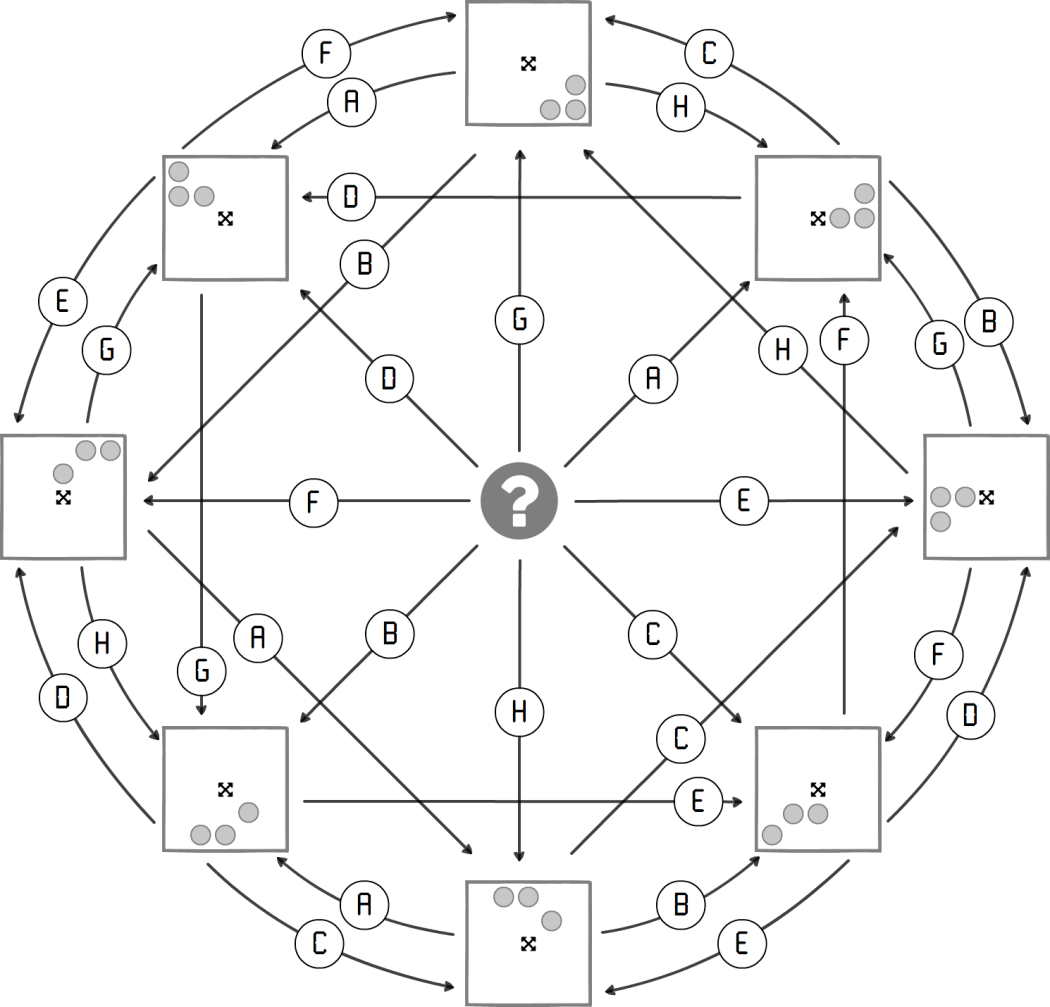
\includegraphics[width=0.78\textwidth]{images/55.png}

「まだ生きている爆発物処理班」の為のヒント:
\begin{itemize}
    \item[$\bullet$] 丸いボタンに色を付けるには、まず右側の色分けボタンを押してから、点灯させたい左側のボタンを押します。
    \item[$\bullet$] 上書きすることで色を変えることができます。色を完全に削除するには、色分けボタンが選択されていない状態で左側のボタンを押してください。色が変更できない場合は、その色が正しいことが既に確認されていることを意味します。
\end{itemize}

\begin{textblock*}{5cm}(16cm,18cm)
\bgroup
\def\arraystretch{1.4}
\begin{tabular}{|c|c|}
    \hline
    文字 & 色 \\ \hline
    A\quad E & 青 \\ \hline
    B\quad F & 黄 \\ \hline
    C\quad G & 赤 \\ \hline
    D\quad H & 緑 \\ \hline
\end{tabular}
\egroup
\end{textblock*}


